\documentclass[14pt]{article}
\usepackage{listings}
\usepackage{color}
\usepackage{graphicx}
\usepackage{setspace}

\definecolor{dkgreen}{rgb}{0,0.6,0}
\definecolor{gray}{rgb}{0.5,0.5,0.5}
\definecolor{mauve}{rgb}{0.58,0,0.82}

\lstset{frame=tb,
  language=java,
  aboveskip=3mm,
  belowskip=3mm,
  showstringspaces=false,
  columns=flexible,
  basicstyle={\small\ttfamily},
  numbers=none,
  numberstyle=\tiny\color{gray},
  keywordstyle=\color{blue},
  commentstyle=\color{dkgreen},
  stringstyle=\color{mauve},
  breaklines=true,
  breakatwhitespace=true
  tabsize=3
}







\begin{document}
\title{% 
  \huge Concurrent and Distributed Systems \\
  \vspace{20mm}
  \large Concurrent Problem Solving Lab Assignment \\}

\date{\today}
\maketitle
\begin{center}
\vspace{30 mm}

\title{\huge Student: Marcu Andrei Cristian}
\\\vspace{10 mm}
\title{\huge Computers and Information Technology}
\\\vspace{10 mm}
\title{\huge CEN 3.2 A}
\\\vspace{10 mm}
\title{\huge 3rd Year}
\end{center}
\date{}
\maketitle

\newpage
\section*{Problems statements}
\vspace{20 mm}
\textbf{Problem 1} (50p) \\
Implement a program to solve the producer-consumer problem using:\\
a) coarse synchronization\\
b) fine synchronization.\\
The code must be tested with at least 4 producers and the number of consumers will be given by the number of available virtual CPUs.
\\\vspace{10 mm}\\
\textbf{Problem 2} (50p) \\
Develop and implement a program to multiply 2 matrices of size 1024x1024 using divide-et-impera.\\
The multiplication of matrices will be realized in a concurrent way using executors and the number of threads will be given by the number of available virtual CPUs.
\begin{center}
\end{center}
\newpage
Both problems are implemented using Java.
\\\vspace{10 mm}\\
\textbf{Problem1:} a) For the coarse implementation I've used only one lock each time a producer/consumer calls the function that modifies the queue. This method is not as efficient as the fine synchronization but it's way safer than that one. We also have two lock conditions "notFull, notEmpty" which are made in order to notify the consumer when the queue is not empty and the producer when the queue is not full\\
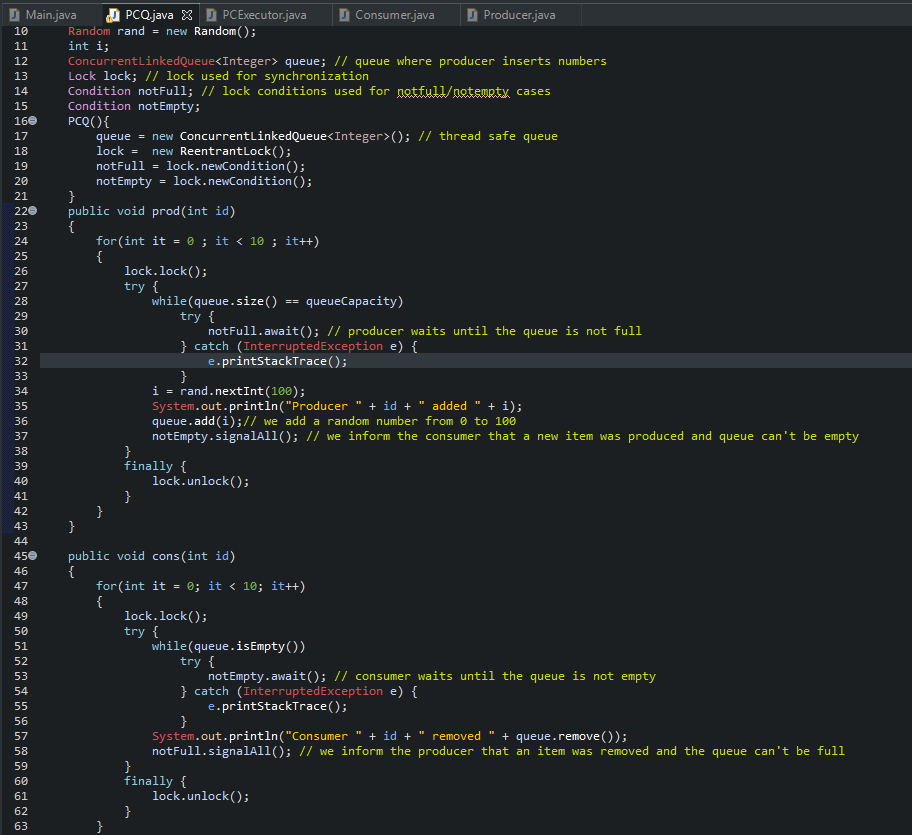
\includegraphics[height=5.8in, width = 5.5in]{coarse.png}\\
\textbf{Problem1:} b) For the fine implementation I've used an array of locks for each elements in queue. This method is more efficient than the coarse implementation but it's harder to get it to work right. I've made an array of conditions too. Both solutions are using the number of available CPUs as threads.\\
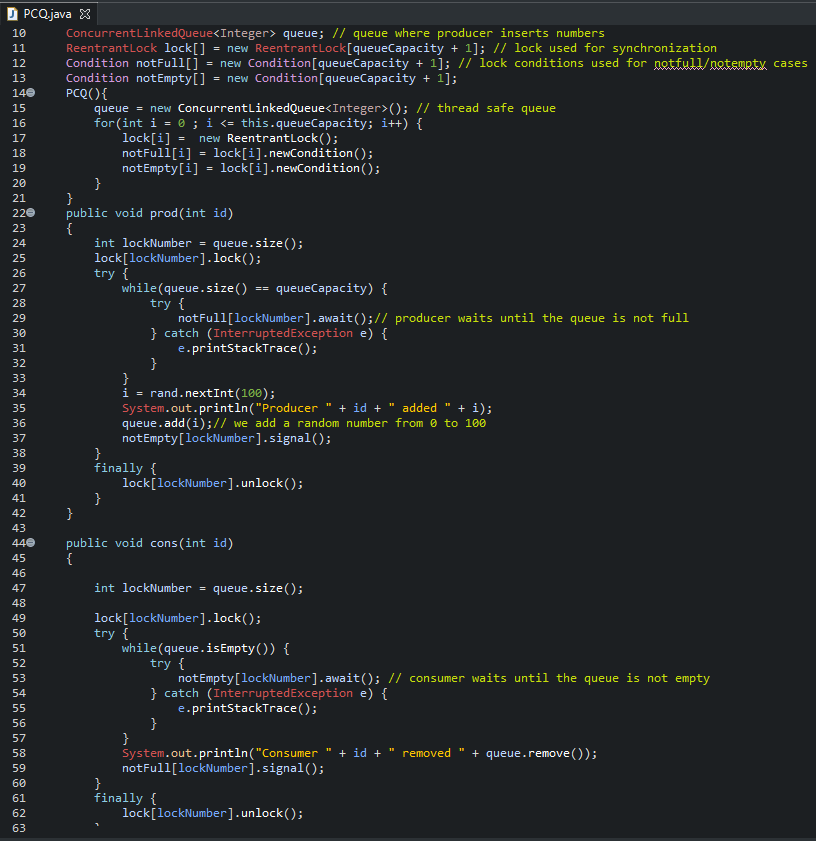
\includegraphics[height=6.2in, width = 5.5in]{fine.png}\\
\\\vspace{20 mm}\\
\section*{Experiments and results for matrix multiplication}
\\\\\\
\begin{center}
Both producer and consumer will run forever. I've printed as much as I could from the execution.\\
1. Example a)\\
\vspace{10mm}

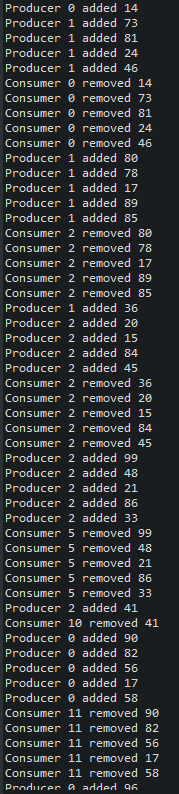
\includegraphics[height=5.5in, width = 2.3in]{coarse1.png}\\
\end{center}\\
\begin{center}
2. Example b)\\
\vspace{10mm}

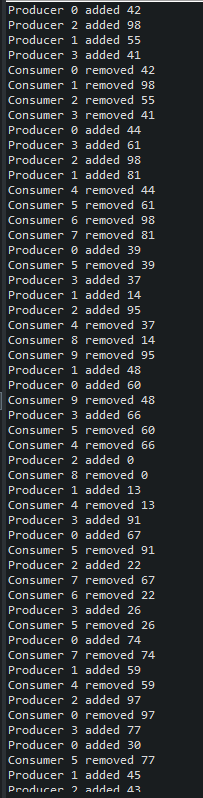
\includegraphics[height=6.5in, width = 2.5in]{fine1.png}\\
\end{center}
\section*{Conclusions Producer Consumer problem}
\vspace{10 mm}
The coarse solution for the problem is more ineffective than the fine solution but it's easier to debug the code and prevent upcoming bugs. The fine method uses more locks and each of them can cause the code go wrong but it is efficient.\\
\newpage
\textbf{Problem2:} In order to solve the divide-et-impera multiplication matrix I've took the add matrix solution presented on the 10th course by our teacher. I've modified the code in order to support multiplication too. In the end the code presented there proved to be way less ineffective than the classical math matrix multiply. In my code I've got both solutions in order to compare them. I've tried to use an exact number of CPUs like it's said in the problem statement but it doesn't work for this solution. I've let it with cached thread pool which is more efficient. I have added two new classes, MathMultiplication which makes the classic math matrix multiplication and MatrixGenerator which generates random matrices. I have also added one method on the Matrix class which prints the matrix\\
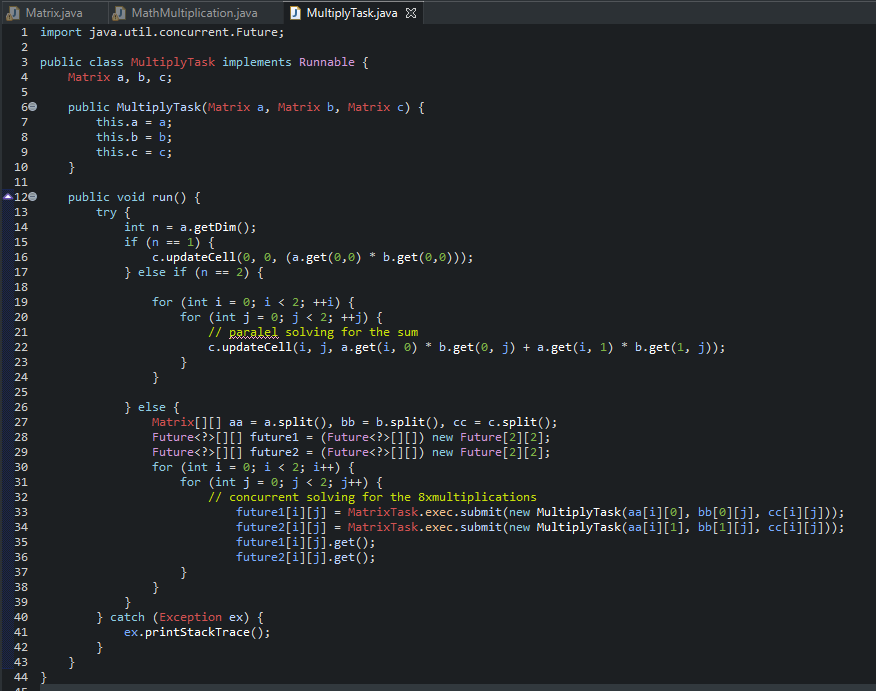
\includegraphics[height=5.5in, width = 5.5in]{matrix1.png}\\
\section*{Experiments and results for producer-consumer}
\\\\\\
\begin{center}
Matrices we want to multiply\\
\vspace{10mm}

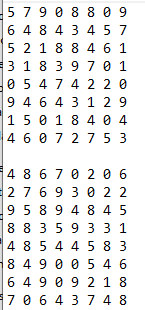
\includegraphics[height=3.5in, width = 2.3in]{result1.png}\\
\end{center}\\
\begin{center}
\newpage
Result\\
\vspace{10mm}

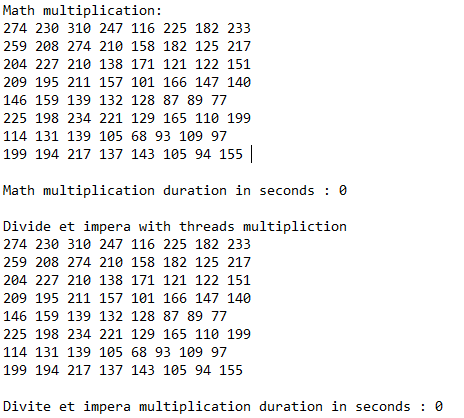
\includegraphics[height=4.5in, width = 2.5in]{result2.png}\\
\end{center}
\section*{Conclusions Matrix multiplication problem}
\vspace{10 mm}
I've used the solution implemented in course, which proved being very slow. In the end the code will compute the result matrix correct but the execution time for the 1024x1024 matrix is somewhere between 2-3 minutes. For the rest it goes in maximum 1 minute. I will present examples in the Experiments and results folder
\section*{References}
https://blog.georgovassilis.com/2014/02/04/on-coarse-vs-fine-grained-synchronization/\\
https://en.wikipedia.org/wiki/Strassen_algorithm\\
www.overleaf.com\\

\end{document}